% PARKED TEXT (not compiled). Preliminary application results written 2026-10-15 from the first analysis of the
% clamping runs; restore and update when all runs and the DFT band gaps are complete.

%% ---- results.tex (former subsections) ----
\subsection{Elastic response}
\label{sec:res-elastic}

The elastic constants obtained from the strain and pressure ladders at the anchored
operating temperature are listed in Table~\ref{tab:elastic}. \MASnI{}, which sits
\SI{25}{K} above its model \Tc{} at this temperature, is the softest in-plane, consistent
with the elastic softening expected near a displacive transition. \FASnI{}, more than
\SI{60}{K} above its tilt transition, is the stiffest. With these biaxial moduli an in-plane
stress of \SI{50}{MPa} corresponds to a biaxial strain of about \SI{0.3}{\percent} in
\CsSnI{}, \SI{0.5}{\percent} in \MASnI{} and \SI{0.14}{\percent} in \FASnI{}, the range of
residual strains measured in films.\cite{Zhao2017SciAdv}
\todo{compare with measured elastic moduli of Sn iodide perovskites}

\begin{table}[htbp]
  \centering
  \caption{Elastic constants of UrsaMLFF + D3 at the anchored operating temperature
    (\CsSnI{} \SI{349}{K}, \MASnI{} \SI{364}{K}, \FASnI{} \SI{303}{K}), fitted to the
    biaxial-strain and hydrostatic-pressure ladders (one run per point).}
  \label{tab:elastic}
  \begin{tabular}{lcccc}
    \toprule
    compound & $Y/(1-\nu)$ (GPa) & $\nu$ & $Y$ (GPa) & $B$ (GPa) \\
    \midrule
    \CsSnI{} & 15.9 & 0.35 & 10.3 & 14.0 \\
    \MASnI{} & 10.0 & 0.28 & 7.2 & 11.4 \\
    \FASnI{} & 36.1 & 0.12 & 31.8 & 14.8 \\
    \bottomrule
  \end{tabular}
\end{table}

\subsection{In-plane strain controls the tilt about the film normal}
\label{sec:res-ladder}

The biaxial ladders show the mechanism by which clamping acts on these films
(Figure~\ref{fig:ladder}a). A tilt about the film normal contracts the in-plane
Sn--Sn distances, so in-plane tension opposes it and in-plane compression favours it. In
\CsSnI{} at \SI{349}{K} the in-phase tilt about the normal falls steadily from
\ang{13.9} at \SI{-2}{\percent} strain to \ang{9.9} in the free crystal and \ang{8.8}
at \SI{+0.5}{\percent}, and collapses between \SI{+0.5}{\percent} and
\SI{+1}{\percent}; at \SI{+2}{\percent} a different pattern with the in-phase axis in the
plane appears. In \MASnI{} at \SI{364}{K} the antiphase tilt about the normal is lost
between \SI{+0.25}{\percent} and \SI{+0.5}{\percent}: a tensile strain of the size measured
in films switches the tilt state of \MASnI{} at its operating point. The free \MASnI{}
crystal itself is bistable at this temperature (one of three runs is untilted, two carry
antiphase tilts of \ang{8.9} and \ang{8.2}), as expected \SI{25}{K} above a transition
whose run-to-run scatter is \SI{29}{K}. In \FASnI{}, which has no tilt order at
\SI{303}{K}, compression induces an in-phase tilt about the normal (\ang{5.0} at
\SI{-2}{\percent}).

The orientation of the molecular cations responds much less
(Figure~\ref{fig:ladder}b). The fraction of FA axes nearest to a pseudo-cubic
$\langle100\rangle$ direction decreases steadily with tension, by 0.06 across the
ladder. The fraction of MA axes near $\langle100\rangle$ (about 0.7) shows no trend beyond
the scatter of the free runs. At the level of these orientation statistics, the response
to strain orders \FASnI{} $>$ \MASnI{}, contrary to our prediction; in \MASnI{} the strain
acts through the octahedral tilt instead.

\begin{figure}[htbp]
  \centering
  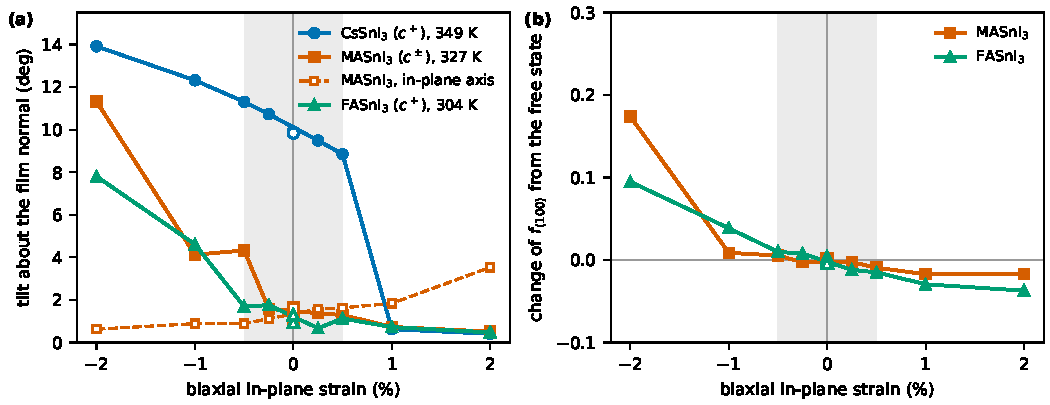
\includegraphics[width=\linewidth]{figures/fig_ladder.pdf}
  \caption{Response to biaxial in-plane strain at the anchored operating temperature
    (filled symbols, one run per strain; $a$ and $b$ fixed, $c$ free). Open symbols: the
    three free runs. Grey band: $\pm\SI{0.5}{\percent}$, the range of measured residual
    strains. (a) Amplitude of the octahedral tilt about the film normal: in-phase ($c^+$)
    for \CsSnI{} and \FASnI{}, antiphase ($c^-$) for \MASnI{}. (b) Change of the fraction
    of cation axes nearest to $\langle100\rangle$, relative to the mean of the free runs
    (\MASnI{} 0.69, \FASnI{} 0.22).}
  \label{fig:ladder}
\end{figure}

\subsection{The three clamping brackets}
\label{sec:res-brackets}

Table~\ref{tab:brackets} summarises the states reached under the three boundary
conditions at the anchored operating temperature. The stress-controlled bracket adds the
intended \SI{50}{MPa} of in-plane tension in all three compounds. It reduces the tilt about
the normal of \CsSnI{} from \ang{9.9} to \ang{9.1} in every run, and that of \MASnI{} on
average from \ang{5.9} to \ang{4.7}, but the \MASnI{} runs scatter as widely as the free
ones.

\begin{table}[htbp]
  \centering
  \caption{States at the anchored operating temperature under the three brackets. $\Delta
    \sigma_\parallel$: mean in-plane stress relative to the free runs (MPa, tensile
    positive). Tilt: amplitude about the film normal (deg; \CsSnI{} and \FASnI{} in-phase,
    \MASnI{} antiphase), mean and individual runs. $f_{\langle100\rangle}$: fraction of
    cation axes nearest to $\langle100\rangle$. Three runs per entry except the \FASnI{}
    rigid clamp (two).}
  \label{tab:brackets}
  \begin{tabular}{llccc}
    \toprule
    compound & bracket & $\Delta\sigma_\parallel$ & tilt (runs) & $f_{\langle100\rangle}$ \\
    \midrule
    \CsSnI{} & free & 0 & 9.9 (9.9, 9.8, 9.8) & -- \\
             & stress-controlled & $+50$ & 9.1 (9.2, 9.1, 9.0) & -- \\
             & rigid clamp & $0$ & 4.1 (1.6, 8.6, 2.2) & -- \\
             & $\gamma$ held under clamp & $+82$ & 7.9 (7.8, 7.8, 8.1) & -- \\
    \MASnI{} & free & 0 & 5.9 (0.7, 8.9, 8.2) & 0.69 \\
             & stress-controlled & $+47$ & 4.7 (6.4, 3.3, 4.4) & 0.69 \\
             & rigid clamp & $+41$ & 3.0 (4.8, 1.3, 2.9) & 0.69 \\
    \FASnI{} & free & 0 & 1.0 (1.5, 1.1, 0.5) & 0.22 \\
             & stress-controlled & $+51$ & 1.1 (1.5, 0.7, 1.0) & 0.22 \\
             & rigid clamp & $+79$ & 0.6 (0.5, 0.8) & 0.16 \\
    \bottomrule
  \end{tabular}
\end{table}

The rigid clamp acts differently in each compound. \CsSnI{} is clamped in the $\beta$
phase at the anneal and crosses the $\gamma\leftrightarrow\beta$ transition on cooling. The
three clamped runs end in three different tilt states: one in the free $\gamma$ pattern with
its in-phase axis along the normal, one with the in-phase axis in the plane, and one with
weak, mixed tilts. Their mean in-plane stress equals that of the free crystal, whereas a
$\gamma$ crystal prepared in the free orientation and then held under the same clamp
carries \SI{82}{MPa} of in-plane tension. The clamp thus selects or frustrates tilt
variants rather than straining a single one: the film relieves the clamping stress by
reorganising its tilt pattern. Which variant forms is decided kinetically at \SI{2}{K/ps},
and the odd in-plane repeat of the production cell ($5\times5$) frustrates the variant with
an in-phase axis in the plane (the section \emph{Limitations}). Clamped at the cubic anneal
(\SI{440}{K} device, \SI{489}{K} model), \CsSnI{} retains no tilt order at the operating
temperature (all amplitudes below \ang{3}). \MASnI{} under the rigid clamp carries a smaller
antiphase tilt on average (\ang{3.0} against \ang{5.9} free), as the ladder predicts for its
in-plane tension, again with large run-to-run scatter. In \FASnI{} the rigid clamp leaves the octahedra untilted but lowers
the fraction of FA axes near $\langle100\rangle$ from 0.22 to 0.16 in both runs, a change
that the strain ladder at comparable strain does not show. It may reflect the cooling
history under the clamp and needs more runs before it is interpreted.
\todo{confirm with additional rigid-clamp runs of \FASnI{}}

The anchoring of the temperatures is essential to these results. At the unshifted device
temperatures (one run per bracket), \CsSnI{} is \SI{111}{K} below its model
$\gamma\leftrightarrow\beta$ transition at \SI{300}{K}. All brackets, including both
rigid-clamp histories, then end in the free $\gamma$ pattern, and an unanchored simulation
would conclude that clamping has no structural effect on \CsSnI{}.

\subsection{Transition temperatures under the clamp}
\label{sec:res-dtc}

Heated under the in-plane clamp of the anneal state, \CsSnI{} loses its second tilted axis
at \SI{404 \pm 4}{K} and all tilt order at \SI{448 \pm 19}{K} (three runs; one run keeps
some order to the top of its ramp at \SI{482}{K}), against \SI{411 \pm 7}{K} and
\SI{462 \pm 17}{K} for the free crystal. The shifts, $\dTc = \SI{-7 \pm 8}{K}$ and
\SI{-14 \pm 25}{K}, are zero within their uncertainty. A clamp set by the anneal-state
cell therefore shifts the $\gamma\leftrightarrow\beta$ transition of \CsSnI{} by less than
about \SI{15}{K} on heating, and the shift of the $\beta\leftrightarrow\alpha$ transition is
not resolved. The structural effect of the clamp is on the tilt variants that form on
cooling.
\todo{Clamped heating ramps for \MASnI{} and \FASnI{}, if added.}

\subsection{Band-gap shifts}
\label{sec:res-deg}

\todo{Results of DFT batch 1 and 2. Batch 1 (sent for DFT on 2026-10-15) contains 124 full
production frames: per compound two frames for the $k$-mesh check, 30 Level-1 frames (six
free frames, each as is and affinely strained to the stress-controlled, rigid-clamp and
$\pm\SI{0.3}{GPa}$ cells) and 8 to 12 pilot frames for the Neyman allocation. To report:
$k$-mesh check; paired $\dEg$ for the stress-controlled and rigid-clamp cells and
$\mathrm{d}\Eg/\mathrm{d}\ln V$; stratified bracket means and fifth percentiles with
standard errors; Level 2 $-$ Level 1; UrsaMLFF energy, force and stress errors on the
production frames.}


%% ---- Limitations items specific to the clamping study ----
  \item \emph{Finite cells.} In the 2000-atom cell of \CsSnI{} ($5\times5\times4$) the odd
    in-plane repeat cannot hold an in-phase tilt about an in-plane axis, which frustrates
    one of the tilt variants that the clamp can select. \todo{repeat the \CsSnI{} rigid-clamp
    runs in the even $6\times6\times4$ cell (2880 atoms)} Domain walls between variants and
    grain boundaries are not represented.
  \item \emph{Statistics.} Three runs per bracket and one run per ladder point; the
    \MASnI{} brackets scatter widely because the operating point lies near \Tc{}.

%% ---- abstract sentences ----
% In-plane tension suppresses
% the octahedral tilt about the film normal; a strain of \SI{0.5}{\percent}, the size measured
% in films, removes the tetragonal tilt of \MASnI{} at its operating point. A clamp set at the
% anneal leaves the transitions of \CsSnI{} unshifted within \SI{15}{K} but selects which tilt
% variants form on cooling. The cation orientations respond weakly, more for formamidinium than
% for methylammonium. \todo{Band-gap result: paired and ensemble gap shifts from DFT on
% stratified samples of the clamped and free ensembles.}
% 
%% ---- former conclusions.tex ----
% % =====================================================================================
% % CONCLUSIONS. Draft: to be completed when the band-gap results (Sec. 3.7) exist.
% % =====================================================================================
% 
% We have simulated films of \CsSnI{}, \MASnI{} and \FASnI{} under the mechanical boundary
% conditions that a substrate imposes after the anneal, with a DFT-trained force field in
% cells of 2000 to 2304 atoms and with temperatures anchored to the model's own transitions.
% The results so far establish four points.
% 
% \begin{enumerate}
%   \item The free-standing crystals follow their experimental phase sequences on heating,
%     but the absolute transition temperatures depend on the dispersion correction and the
%     functional by of order \SI{100}{K}. Anchoring the simulation temperatures to the model's
%     \Tc{} changes the outcome qualitatively: without it, clamped \CsSnI{} shows no structural
%     response at all.
%   \item In-plane strain acts on the octahedral tilt about the film normal. Tension
%     suppresses it and compression enhances it; a tension of \SI{0.25}{\percent} to
%     \SI{0.5}{\percent}, the size of measured residual strains, removes the tetragonal tilt of
%     \MASnI{} at its operating point.
%   \item A rigid clamp set at the anneal does not measurably shift the
%     $\gamma\leftrightarrow\beta$ transition of \CsSnI{} on heating
%     (\SI{-7 \pm 8}{K}), but it changes which tilt variants form on cooling, and the film
%     relieves the clamping stress by reorganising its tilt pattern.
%   \item The orientation statistics of the molecular cations respond weakly to strain, more
%     for FA than for MA, contrary to the predicted ordering; in \MASnI{} the strain acts
%     through the octahedral framework.
% \end{enumerate}
% 
% \todo{Band-gap conclusions: the paired (elastic) and ensemble gap shifts per compound and
% bracket, the tilt and orientation contribution, the low-gap tail, and the device implication
% of the anneal temperature as a manufacturing variable.}

%% ---- Limitations subsection (removed from conclusions.tex on 2026-10-15, user: 'remove limitations section for now') ----
\subsection*{Limitations}
\label{sec:limitations}

\begin{itemize}
  \item \emph{No spin--orbit coupling.} Only gap differences between matched states are
    reported, under the assumption that the SOC correction is the same in both states
    (the section \emph{Electronic structure}). No absolute gap is claimed. \todo{decide whether to include
    the SOC benchmark of the earlier workflow (PBE vs PBE+SOC on a 384-atom \MASnI{} cell,
    legacy draft) as a size estimate of the correction}
  \item \emph{Semilocal gaps.} PBEsol underestimates band gaps; differences between similar
    structures are expected to be more reliable than absolute values, but a second gap
    estimator has not been applied.
  \item \emph{Force field.} UrsaMLFF under-stabilises the tilted phases of \CsSnI{}, and its
    MD of the hybrids leaves its training data (the section \emph{Accuracy of the force field}). The absolute
    transition temperatures depend on D3 and on the functional by of order \SI{100}{K};
    the anchoring of temperatures and the restriction to differences address this but do
    not remove it, and no second functional was used for the clamping study.
  \item \emph{Kinetics.} The model supercools by 60 to \SI{120}{K} on cooling at
    \SI{2}{K/ps}; transition temperatures are therefore quoted on heating.
  \item \emph{Out of scope.} Grain boundaries, Sn vacancies and Sn$^{2+}$ oxidation,
    surfaces and interfaces, and ion migration on time scales of seconds to hours.
\end{itemize}
